\documentclass{cours}

\usepackage{tikz}
\usetikzlibrary{arrows.meta}

\title{Continuité des Fonctions \\ d'une Variable Réelle}
\author{Diego Van Overberghe}

\begin{document}
    \maketitle{2}

    \begin{Gpartie}{Définition}
        Soit $f$, définie sur un intervalle $I$, et soit $a$, un réel de $I$.
        La fonction $f$ est \emph{continue} si et seulement si : \[\boxed{\lim_{x \to a} f(x)=f(a)}\]
        $f$ est continue sur l'intervalle $I$, si et seulement si, quel que soit le réel $x\in I$, $f$ est continue en $x$.

        H.P.: $\quad\forall\epsilon >0,~\exists\alpha >0,~\forall x\in\big]~a-\alpha~;~a+\alpha~\big[,~f(x)\in\big]~f(a)-\epsilon~;~f(a)+\epsilon~\big[$
        \begin{Spartie}{Exemple}
            La fonction inverse est continue sur $\big]-\infty\,~;~0\,\big[$, et sur $\big]\,0\,~;~+\infty\,\big[$.

            La fonction \og Partie Entière \fg{} est définie sur $\mathbb{R}$, mais pas continue sur $\mathbb{R}$.
            \vspace{1ex}
            \begin{center}\begin{tikzpicture}[scale=0.7]
                \begin{axis}[
                    xmin=-0.5,  xmax=3.5,
                    ymin=-0.5,  ymax=3.5,
                ]
                    \addplot[color=blue, very thick, jump mark left, samples=5, mark=*, domain=0:4]{floor(x)};
                \end{axis}
            \end{tikzpicture}\end{center}
            \parbox{\linewidth}{\captionof{figure}{\centering Représentation Graphique de la Fonction \og Partie Entière \fg{}, continue sur $\big[n\,~;~n+1\,\big[$ avec $n\in\mathbb{Z}$.}}
            \vspace{1ex}
            \begin{center}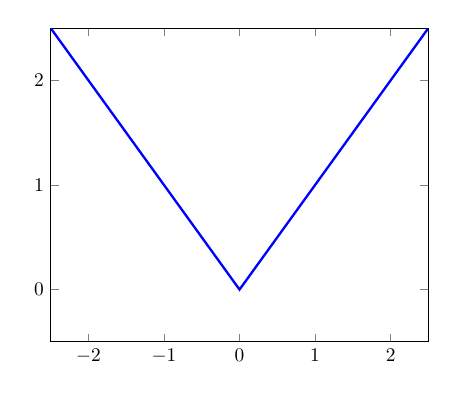
\begin{tikzpicture}[scale=0.7]
                \begin{axis}[
                    xmin=-2.5,  xmax=2.5,
                    ymin=-0.5,  ymax=2.5,
                ]
                    \addplot[color=blue, very thick]{abs(x)};
                \end{axis}
            \end{tikzpicture}\end{center}
            \parbox{\linewidth}{\captionof{figure}{Représentation Graphique de la Fonction Absolue, continue sur $\mathbb{R}$}}
        \end{Spartie}
        \begin{Spartie}{Propriété}
            La somme, le produit et la composée de deux fonctions continues est continue. \\
            L'inverse d'une fonction continue est continue sur tout intervalle où elle ne s'annule pas.
            \[f : x\mapsto x^2\quad\text{continue}\] \[g : x\mapsto\dfrac{1}{x^2}\quad\text{Définie sur }\mathbb{R}^*\text{, continue sur }\big]-\infty\,~;~0\,\big[\text{ et }\big]\,0\,~;~+\infty\,\big]\]
        \end{Spartie}
    \end{Gpartie}

    \hspace{4ex}

    \begin{Gpartie}{Théorème des Valeurs Intermédiaires}
        \begin{Spartie}{Théorème}
            Si une fonction $f$ est continue sur un intervalle $\big[a\,~;~b\,\big]$ alors, pour tout réel $k\in\Big[\mathrm{min}\,\big(f(a)\,~;~f(b)\,\big)\,~;~\mathrm{max}\,\big(f(a)\,~;~f(b)\,\big)\Big]$, il existe \emph{au moins} un réel $c\in\big[a\,~;~b\,\big]$, tel~que $f(c)=k$.

            C'est-à-dire, pour tout réel $k$, compris entre $f(a)$ et $f(b)$, il existe un réel $c\in\big[a\,~;~b\,\big]$, tel que $f(c)=k$.
            \begin{center}
                \begin{tikzpicture}[
                    scale=1.5,
                    % dot/.style={
                    %     draw=black,
                    %     fill=darkgray,
                    %     circle,
                    %     minimum size=2pt,
                    %     inner sep=0pt,
                    %     solid,
                    % },
                ]
                    \begin{axis}[
                        xmin=-5,    xmax=5,
                        ymin=-1,    ymax=5,
                        xtick=\empty,
                        ytick=\empty,
                        domain=-4.9:2.85
                    ]
                        \addplot[color=blue, very thick, samples=50, name path=func]{0.1*x^3+0.3*x^2-0.5*x+1} node[below right]{$\mathcal{C}_f$};
                        \draw[dashed, red, thick]
                            ( -3.6,2 ) -- (-1.4,2) -- (2,2) node [dot, label={[label distance=-2pt]0:$k$}] {}
                            ( -3.6,2 ) node [dot] {} -- (-3.6,0) node [label={[label distance=-6pt]270:$c_1$}] {}
                            ( -1.4,2 ) node [dot] {} -- (-1.4,0) node [label={[label distance=-6pt]270:$c_2$}] {}
                            ( 2,2 ) node [dot] {} -- (2,0) node [label={[label distance=-6pt]270:$c_3$}] {};

                        \draw[dashed, black, thick]
                            (0,4) node [label=left:$f(b)$] {} -- (2.75,4) node [dot] {} -- (2.75,0) node [label=below:$b$] {}
                            (-4.75,0) node [label=above:$a$] {} -- (-4.75,-0.6) node [dot] {} -- (0,-0.6) node [label=right:$f(a)$] {};
                    \end{axis}
                \end{tikzpicture}
                \parbox{\linewidth}{\captionof{figure}{Présentation du Théorème des Valeurs Intermédiaires}}
            \end{center}
            Pour tout $k$ appartenant à $\big[f(b)\,~;~f(a)\,\big]$, il existe au moins un réel $c\in\big[a\,~;~b\,\big]$, tel que $f(c)=k$.
        \end{Spartie}
        \pagebreak
        \begin{Spartie}{Corollaire}
            Si une fonction $f$ est \textit{continue} et \textit{strictement monotone} sur un intervalle $\big[a\,~;~b\,\big]$, alors, pour tout $k\in\Big[\mathrm{min}\,\big(f(a)\,~;~f(b)\,\big)\,~;~\mathrm{max}\,\big(f(a)\,~;~f(b)\,\big)\Big]$, il existe un \textit{unique} réel $c\in\big[a\,~;~b\,\big]$, tel que $f(c)=k$. 
            \begin{center}
                \begin{tikzpicture}[scale=1.5]
                    \begin{axis}[
                        xmin=-0.5,  xmax=1.5,
                        ymin=-0.5,  ymax=2.5,
                        xtick=\empty,
                        ytick=\empty,
                        domain=-0.25:1.05
                    ]
                        \addplot[color=blue, very thick, samples=20]{x^3+x};

                        \draw[dashed, red, thick]
                            (0,1.05) node [label={[label distance=-2pt]180:$k$}] {} -- (0.7,1.05) node [dot] {} -- (0.7,0) node [label={[label distance=-2pt]270:$c$}] {};

                        \draw[dashed, black, thick]
                            (0,0.21) node [label={[label distance=-2pt]180:$f(a)$}] {} -- (0.2,0.21) node [dot] {} -- (0.21,0) node [label={[label distance=-2pt]270:$a$}] {}
                            (0,2) node [label={[label distance=-2pt]180:$f(b)$}] {} -- (1,2) node [dot] {} -- (1,0) node [label={[label distance=-4.5pt]270:$b$}] {};
                    \end{axis}
                \end{tikzpicture}
                \parbox{\linewidth}{\captionof{figure}{\centering Illustration du Corollaire du Théorème \linebreak des Valeurs Intermédiaires}}
            \end{center}
            \begin{SSpartie}{Cas Particulier}
                Si une fonction $f$ est continue sur un intervalle $\big[a\,~;~b\,\big]$, et si $f(a)$ et $f(b)$ sont de signes contraires, il existe au moins une solution à $f(x)=0$, sur $\big[a\,~;~b\,\big]$.
            \end{SSpartie}
        \end{Spartie}
    \end{Gpartie}
\end{document}